\chapter{Theory and Motivation}

The Standard Model (SM) of particle physics is our current best theory to describe the fundamental particles and their interactions.
The SM describes the strong force, as well as unifying the weak and electromagnetic forces.
The latter is partly done through the Brout-Englert-Higgs (BEH) mechanism for spontaneous symmetry breaking, that allows many fundamental particles to obtain masses.
It also predicts a new scalar boson, named the Higgs boson.
In 2012, the ATLAS \cite{ATLAS_Higgs_Discovery} and CMS collaboration \cite{CMS_Higgs_Discovery} discovered a Higgs boson-like particle when colliding protons at high energy at the Large Hadron Collider (LHC) and further measurements of this particle's properties have been consistent with such a particle.
This discovery experimentally completed the SM particle constituents. \\

However, the SM is not without theoretical problems and experimental tensions.
Firstly, the hierarchy problem describes the issue of lightness of the observed Higgs boson mass and the "unnatural" balancing of inputs needed to explain the theorised loop corrections to the predicted mass. 
These are orders of magnitude larger than then observed mass.
A solution to this problem is Supersymmetry, but no experimental evidence for this theory has yet been found that separates it from the SM. 
Secondly, results from the LHCb experiment \cite{LHCb:2021trn,Kowalewski:2013mna,BaBar:2013mob,Belle:2015qfa,LHCb:2015gmp,Belle:2016dyj,LHCb:2017rln,LHCb:2017smo} and the g−2 experiment \cite{Muong-2:2021ojo} have shown deviations from the SM predictions.
Although not the statistical significance for a discovery, they offer intriguing hints at potential Beyond SM (BSM) physics.
BSM particles, produced from extended Higgs sectors or otherwise, have been theorised to explain these deviations .
This chapter will explain the SM and the Higgs sector theory, as well as detailing the BSM extensions that can help resolve the theoretical tensions and experimental tensions.

\section{The Standard Model of Particle Physics}

\subsection{Fundamental Particles and Interactions}

The SM is a set of fundamental particles, as shown in Figure~\ref{fig:sm_diagram}, and rules that govern the interactions between particles.
The interactions between these particles are able to model the strong, weak and electromagnetic force, unifying the later two into one electroweak interaction.
The SM consists of 6 quarks, 3 charged leptons and 3 neutrinos, which are grouped in fermions because of their shared half integer spin. 
Each of these particles contain an anti-partner with opposite quantum numbers but the same mass.
The SM also consists of a number of bosons (integer spin) that describe the fundamental forces of nature: the strong, weak, and electromagnetic forces. 
The gluon is the mediator of the strong force, the W and Z bosons mediate the weak force, and the photon mediates the electromagnetic force. \\

\begin{figure}[!hbtp]
\centering
    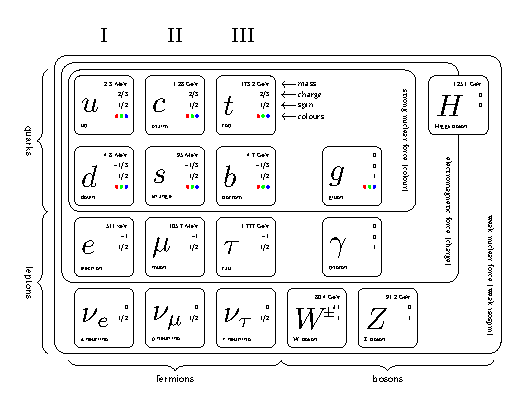
\includegraphics[width=\textwidth]{Figures/SM_diagram.pdf}
\caption{Diagram of the fundamental particles the constitute the SM. Also displayed are the fermion generation shown in Roman numerals, the particles measured mass, charge, spin and colours available for the strong interaction. This is taken and adjusted from Ref.~\cite{}}
\label{fig:sm_diagram}
\end{figure}

The SM is a renormalisable quantum field theory that is built on the principle of local gauge invariance.
The SU(3)$_{\text{C}}$ $\otimes$ SU(2)$_{\text{L}}$ $\otimes$ U(1)$_{\text{Y}}$ is the gauge symmetry group of the SM.
This means that the Lagrangian, that governs the particles interactions, is invariant under such a transformation. 
SU(2)$_{\text{L}}$ $\otimes$ U(1)$_{\text{Y}}$ is the symmetry of the electroweak unification and SU(3)$_{\text{C}}$ is the symmetry of the theory for strong force, name Quantum Chromodynamic (QCD). \\

SOME STUFF ABOUT QCD HERE \\
ALSO MAYBE SOME STUFF ABOUT WHY SU(2)L AND NOT JUST SU(2) \\


Electroweak unification was initially proposed by Glashow~\cite{}, Weinberg~\cite{} and Salam~\cite{} to combine the theories for the weak and electromagnetic forces into one.
It is built on the premise of the Dirac equation.
The Dirac Lagrangian for a massless field, $\psi$, is shown below.

\begin{equation}
\mathcal{L}_{\text{Dirac}} = i\bar{\psi}\gamma^{\mu} \partial_{\mu} \psi
\end{equation}

The SU(2)$_{\text{L}}$ transformation operates on the weak isospin, $I$, only for the left handed spinors and the U(1)$_{\text{Y}}$ transformation operates on the weak hypercharge, $Y=2(Q-I_{3})$, where Q is the charge of the fundamental particles and $I_3$ is the third component of the weak ispospin.
By invoking gauge invariance of the Dirac Lagrangian under such a transformation, four associated gauge fields are present, $\boldsymbol{W}_{\mu} = (W^{1}_{\mu},W^{2}_{\mu},W^{3}_{\mu})$ and $B_{\mu}$.

\begin{align}
\begin{split}
\mathcal{L}_{\text{Electroweak}} &= \bar{\psi}_{L}\Big(\partial_{\mu} + \frac{i}{2} g \boldsymbol{W}_{\mu} \cdot \boldsymbol{\sigma} + g^{\prime} Y B_{\mu}  \Big) \psi_L \\
&+ \bar{\psi}_{R}\Big(\partial_{\mu} + + g^{\prime} Y B_{\mu}  \Big) \psi_R - \frac{1}{4} \boldsymbol{W}_{\mu\nu} \cdot \boldsymbol{W}^{\mu\nu} - \frac{1}{4}B_{\mu\nu}B^{\mu\nu},
\end{split}
\end{align}

where the partial derivatives have been replaced with the covariant derivative and the added field tensors $\hat{\boldsymbol{W}}_{\mu\nu}$ and $\hat{B}_{\mu\nu}$ that are defined as,

\begin{equation}
\boldsymbol{W}_{\mu\nu} = \partial_{\mu} \boldsymbol{W}_{\nu} - \partial_{\nu} \boldsymbol{W}_{\mu} - ig[\boldsymbol{W}_{\mu},\boldsymbol{W}_{\nu}]
\end{equation}

\begin{equation}
B_{\mu\nu} = \partial_{\mu} B_{\nu} - \partial_{\mu} B_{\mu}.
\end{equation}

These fields can be rotated in physical fields for the photon, Z and W boson with the following transformations,

\begin{align}
\begin{split}
W^{\pm}_{\mu} &= \frac{1}{\sqrt{2}}(W^{1}_{\mu} \mp W^{2}_{\mu}), \\
Z_{\mu} &= W^{3}_{\mu} \cos\theta_{w} - B_{\mu} \sin\theta_w, \\
A_{\mu} &= W^{3}_{\mu} \sin\theta_{w} - B_{\mu} \cos\theta_w,
\end{split}
\label{eqn:rotations}
\end{align}

where $\theta_w$ represents the weak mixing angle and is defined such that

\begin{equation}
\sin\theta_w = \frac{g^{\prime}}{\sqrt{g^2 + g^{\prime 2}}}, \hspace{1cm} \cos\theta_w = \frac{g}{\sqrt{g^2 + g^{\prime 2}}}.
\end{equation}

The W$^{\pm}$ and Z bosons were discovered by the UA1 and UA2 collaborations in 1983, which confirmed the predictions made by electroweak unification.
However, the W$^{\pm}$ and Z bosons were measured to have a non-zero mass and Lagrangian mass terms of the form $\frac{1}{2}m_{Z}^2 Z_{\mu} Z^{\mu}$ or $m_{W}^2 W_{\mu}^{-}W^{+\mu}$ cannot be included as they are not invariant under the SU(2)$_{\text{L}}$ $\otimes$ U(1)$_{\text{Y}}$ gauge symmetry.
The same issue also exist in massive fermions, as the fermion mass terms left- and right-handed chiral states, $m\bar{\psi}\psi = m(\bar{\psi}_R \psi_L + \bar{\psi}_L \psi_R)$,  transform differently and therefore does not remain invariant under the gauge transformation.
To resolve this, the Brout-Englert-Higgs (BEH) mechanism for spontaneous symmetry breaking was theorised.

\subsection{Higgs Sector}

The BEH mechanism was proposed in the 1960s by Englert and Brout~\cite{Englert:1964et}, Higgs~\cite{Higgs:1964ia,Higgs:1964pj,Higgs:1966ev} and Guralnik, Hagen and Kibble~\cite{Guralnik:1964eu,Kibble:1967sv}.
It works on the principles of spontaneous symmetry breaking of the SU(2)$_{\text{L}}$ $\otimes$ U(1)$_{\text{Y}}$ gauge symmetry.
It does this by introducing a gauge invariant field that has a non-zero vacuum expectation value (VEV).
The formalism of this is shown below, starting from a complex scalar doublet, $\Phi$. 

\begin{equation}
	\Phi = 
	\begin{pmatrix} 
		\phi^{+} \\
		\phi^{0} \\
	\end{pmatrix},
\end{equation}

where $\phi^{+}$ and $\phi^{0}$ are complex functions.
The Lagrangian and the potential, chosen to fulfil the conditions stated above, then takes the form,

\begin{equation}
	\mathcal{L} = (\partial_{\mu}\Phi)^{\dagger} (\partial^{\mu}\Phi) - V(\Phi)
\end{equation}

with,

\begin{equation}
V(\phi) = \mu^2 \Phi^{\dagger} \Phi + \lambda (\Phi^{\dagger} \Phi)^2,
\end{equation}

where $\mu^2$ and $\lambda$ are two real parameters, $\lambda$ is required to be positive for the vacuum to be stable.
If $\mu^2$ is negative, $\Phi$ will have a non-zero VEV and the field will be able to spontaneously breaking the gauge symmetry.
In the vacuum state, the field must satisfy the criteria,

\begin{equation}
\Phi^{\dagger} \Phi = -\frac{\mu^2}{2\lambda}.
\end{equation}

This potential fulfils the criteria of a non-zero VEV as $\Phi$ must be non-zero. 
Choosing a gauge, to remove the massless scalar bosons predicted by Goldstone's theorem~\cite{Goldstone:1961eq}, by taking $\phi^+$ to be zero and $\phi$ to be real.
The ground state of $\Phi$ is found as,

\begin{equation}
\braket{0|\Phi|0} = \frac{1}{\sqrt{2}}
	\begin{pmatrix} 
		0 \\
		\nu \\
	\end{pmatrix},
\end{equation}

where $\nu^2 = \mu^2 / \lambda$, where $\nu$ is the non-zero VEV.
The complex doublet can then be written as an expansion around the minimum of the potential,

\begin{equation}
\Phi = \frac{1}{\sqrt{2}}
	\begin{pmatrix} 
		0 \\
		\nu + h(x)\\
	\end{pmatrix}
\end{equation}

Applying the covariant derivative for the electroweak gauge symmetry to produce a kinematic term for the field, $\Phi$, yields

\begin{align}
\begin{split}
(D_{\mu}\Phi)^{\dagger} (D^{\mu}\Phi) &= \frac{1}{2}(\partial_{\mu}h)(\partial^{\mu}h) + \frac{1}{8} g^{2} (W_{\mu}^{1} + i W_{\mu}^{2})(W^{1\mu} - i W^{2\mu})(\nu + h)^2 \\
&+ \frac{1}{8} (g W_{\mu}^{3} - g' B_{\mu})(g W^{3\mu} - g' B^{\mu})(\nu + h)^2.
\end{split}
\end{align}

The Lagrangian incorporating this term, gives mass terms for $W_{\mu}^{1}$ and $W_{\mu}^{2}$ and hence the mass of the W boson is $m_W = \frac{1}{2}g\nu$.
Once again the remaining states need to be rotated to give the photon and the Z boson fields.
Setting up the non-diagonal mass matrix for the fields $W_{\mu}^{3}$ and $B_{\mu}$ and calculating the eigenvalues to find the diagonal basis, masses of two fields are found, one equal to 0 and the other equal to $\frac{1}{2} \nu \sqrt{g^2 + g^{\prime 2}}$ which represent the photon and Z boson mass respectively.
The transformation to the photon and Z fields as parametrised in Eq.~\ref{eqn:rotations} utilises,

\begin{equation}
\tan\theta_W = \frac{g^{\prime}}{g}.
\end{equation}

A mass term for the Higgs boson also arises from the potential of the BEH mechanism with $m_h = \sqrt{-2\mu^2}$. 
The same mechanism can also be used to add mass terms for quarks and charged leptons.
Gauge invariant couplings to the Higgs bosons and fermion mass terms can be generated from the BEH mechanism applied to a Lagrangian term of the form,

\begin{equation}
\bar{\psi}_{L}\Phi\psi_{R} + \bar{\psi}_{R}\Phi\psi_{L}.
\end{equation}


\section{Extended Higgs Sector}

There is no theoretical limitation to only have one Higgs doublet in the theory.
Therefore, a natural extension to the SM Higgs sector is the two Higgs doublet model (2HDM).
2HDMs predict 5 Higgs bosons; 1 lighter and 1 heavier scalar ($h$ and $H$), 1 pseudoscalar ($A$) and 2 charged particles ($H^\pm$).
The Lagrangian for such a theory is shown below.

\begin{equation}
\begin{aligned}
\mathcal{L}^{\text{2HDM}}_{\text{yukawa}} &= - \sum_{f=u,d,l}\Big(\frac{m_{f}}{\nu}g^{f}_{h}\bar{f}fh + \frac{m_{f}}{\nu}g^{f}_{H}\bar{f}fH -i\frac{m_{f}}{\nu}g^{f}_{A}\bar{f}\gamma_{5}fA\Big)  \\ 
&- \Big[\frac{\sqrt{2}V_{ud}}{\nu}\bar{u}(m_{u}g^{u}_{A}P_{L} + m_{d}g^{d}_{A}P_{R})dH^{+} + \frac{\sqrt{2}m_{l}g^{d}_{A}}{\nu}\bar{\nu}_{L}l_{R}H^{+} + h.c.\Big],
\end{aligned}
\end{equation}

where $u$, $d$ and $l$ represent up-like quarks, down-like quarks and charged leptons.
$m_{f}$ are the fermion masses, $\nu$ is the vacuum expectation value of the SM Higgs doublet, $g$ are the couplings (relative to the SM couplings) of fermion fields, f, to Higgs fields, $h$, $H$, $A$ and $H^+$.
NEED TO WRITE ABOUT THE OTHER PARAMETERS I DON'T CARE ABOUT ALSO.
There are four main types of 2HDM that are dependent on which Higgs doublet couples to which group of fermions, named type I, II, X (lepton-specific) and Y (flipped).
The couplings of the fermion groups to the Higgs doublets are shown in Tab.~\ref{tab:2hdm_doublets}, by convention $\Phi_2$ is chosen to couple to up-like quarks.

\begin{table}[H]
    \centering
    \begin{tabular}{|x{1.0cm}|x{2.0cm}x{2.0cm}x{2.0cm}x{2.0cm}|}
    		\hline
    	 	& Type I & Type II & Type X & Type Y \\
    	 	\hline
    	 	\hline
    	 	$u$ & $\Phi_2$ & $\Phi_2$  & $\Phi_2$  & $\Phi_2$  \\ 
    	 	$d$ & $\Phi_2$ & $\Phi_1$ & $\Phi_2$ & $\Phi_1$ \\
    	 	$l$ & $\Phi_2$ & $\Phi_1$   & $\Phi_1$    & $\Phi_2$ \\
        \hline
    \end{tabular}
    \caption{Table showing which Higgs doublet different fermion groups different types of 2HDMs couple to. By convention the $u$ quark is chosen to couple to $\Phi_2$.}
    \label{tab:2hdm_doublets}
\end{table}

The type of 2HDM determines the formulae for the couplings, $g$, that are functions on two parameters: the CP-even ($\alpha$) and CP-odd mixing angles ($\beta$).
These relative couplings are shown in Tab.~\ref{tab:2hdm_couplings}.

\begin{table}[H]
    \centering
    \begin{tabular}{|x{1.0cm}|x{2.0cm}x{2.0cm}x{2.0cm}x{2.0cm}|}
    		\hline
    	 	& Type I & Type II & Type X & Type Y \\
    	 	\hline
    	 	\hline
    	 	$g_{h}^{u}$ & $c_{\alpha}/s_{\beta}$ & $c_{\alpha}/s_{\beta}$  & $c_{\alpha}/s_{\beta}$  & $c_{\alpha}/s_{\beta}$  \\ 
    	 	$g_{h}^{d}$ & $c_{\alpha}/s_{\beta}$ & $-s_{\alpha}/c_{\beta}$ & $c_{\alpha}/s_{\beta}$  & $-s_{\alpha}/c_{\beta}$ \\
    	 	$g_{h}^{l}$ & $c_{\alpha}/s_{\beta}$ & $-s_{\alpha}/c_{\beta}$ & $-s_{\alpha}/c_{\beta}$ & $c_{\alpha}/s_{\beta}$  \\
    	 	\hline
    	 	$g_{H}^{u}$ & $s_{\alpha}/s_{\beta}$ & $s_{\alpha}/s_{\beta}$ & $s_{\alpha}/s_{\beta}$ & $s_{\alpha}/s_{\beta}$ \\
    	 	$g_{H}^{d}$ & $s_{\alpha}/s_{\beta}$ & $c_{\alpha}/c_{\beta}$ & $s_{\alpha}/s_{\beta}$ & $c_{\alpha}/c_{\beta}$ \\
    	 	$g_{H}^{l}$ & $s_{\alpha}/s_{\beta}$ & $c_{\alpha}/c_{\beta}$ & $c_{\alpha}/c_{\beta}$ & $s_{\alpha}/s_{\beta}$ \\
    	 	\hline
    	 	$g_{A}^{u}$ & $1/t_{\beta}$ & $1/t_{\beta}$ & $1/t_{\beta}$  & $1/t_{\beta}$ \\
    	 	$g_{A}^{d}$ & $1/t_{\beta}$ & $t_{\beta}$   & $-1/t_{\beta}$ & $t_{\beta}$ \\
    	 	$g_{A}^{l}$ & $1/t_{\beta}$ & $t_{\beta}$   & $t_{\beta}$    & $-1/t_{\beta}$ \\
        \hline
    \end{tabular}
    \caption{Table showing the couplings of fermion groups to additional neutral Higgs bosons in different types of 2HDMs. These are dependent on the mixing angles $\alpha$ and $\beta$. $t_{x}$, $s_{x}$ and $c_{x}$ represent $\tan x$, $\sin x$ and $\cos x$ respectively.}
    \label{tab:2hdm_couplings}
\end{table}

In the alignment limit, for the normal scenario $h_{SM}=h$, $sin(\beta-\alpha)=1$, $\implies$ $c_{\alpha}/s_{\beta}=1$, $s_{\alpha}/c_{\beta}=-1$, $s_{\alpha}/s_{\beta}=-1/t_{\beta}$, $c_{\alpha}/c_{\beta}=t_{\beta}$.

In the alignment limit, for the inverted scenario $h_{SM}=H$, $cos(\beta-\alpha)=1$ $\implies$ $c_{\alpha}/s_{\beta}=1/t_{\beta}$, $s_{\alpha}/c_{\beta}=t_{\beta}$, $s_{\alpha}/s_{\beta}=1$, $c_{\alpha}/c_{\beta}=1$.


\section{Theoretical Problems and Potential Solutions}

\subsection{Hierarchy Problem}

The current best measurement for the SM Higgs boson’s mass from the CMS experiemnt is 125.38 $\pm$ 0.14 GeV~\cite{CMS:2020xrn}.
The lightness is a concern when considering "naturalness" and physics beyond the SM. 
The Higgs boson has loop corrections to calculations of its mass. 
Known heavy fermions already provide significant contributions (orders of magnitude greater than the observed mass) to the Higgs boson’s calculated mass. 
On top of this, treating the SM as an effective field theory, new physics would be expected in the unexplored regions between the weak scale and the Planck scale
But if a new fermion were to be found, $f$, or a heavy scalar, $S$, in such a range, the Higgs boson would be subject to even greater changes in its predicted mass. 
The Feynman diagrams for the mass corrections for a fermion and a scalar are shown in Fig.~\ref{fig:Higgs_One_Loop_Corrections}.

\begin{figure}[H]
\centering
    \begin{subfigure}[b]{0.4\textwidth}
    \centering
    \scalebox{0.8}{
    \begin{tikzpicture}
    \begin{feynman}
    \vertex (a) {\(H\)};
    \vertex [right = 1.5cm of a] (b);
    \vertex [right = 1cm of b] (dummy);
    \vertex [right = 1cm of dummy] (c);
    \vertex [above = 1cm of dummy] (e);
    \vertex [below = 1cm of dummy] (f);
    \vertex [right = 1.5cm of c] (d) {\(H\)};
    \diagram* {
    (a) -- [scalar] (b),
    (b) -- [out=90, in=180] (e),
    (e) -- [out=0, in=90, edge label=\(f\)] (c),
    (b) -- [out=-90, in=180] (f),
    (f) -- [out=0, in=-90] (c),
    (c) -- [scalar] (d)
    };
    \end{feynman}
    \end{tikzpicture}
    }
    \caption{}
    \label{fig:corr_fermion}
    \end{subfigure}
    \begin{subfigure}[b]{0.4\textwidth}
    \centering
    \scalebox{0.8}{
    \begin{tikzpicture}
    \begin{feynman}
    \vertex (a) {\(H\)};
    \vertex [right = 2cm of a] (b);
    \vertex [right = 2cm of b] (c) {\(H\)};
    \vertex [above = 1cm of b] (dummy);
    \vertex [left = 1cm of dummy] (d);
    \vertex [above = 1cm of dummy] (e);
    \vertex [right = 1cm of dummy] (f);
    \diagram* {
    (a) -- [scalar] (b),
    (b) -- [scalar, out=180, in=-90] (d),
    (d) -- [scalar, out=90, in=-180] (e),
    (e) -- [scalar, out=0, in=90, edge label=S] (f),
    (f) -- [scalar, out=-90, in=0] (b),
    (b) -- [scalar] (c)
    };
    \end{feynman}
    \end{tikzpicture}
    }
    \caption{}
    \label{fig:corr_scalar}
    \end{subfigure}
    \caption{One-loop corrections to the Higgs mass by a fermion f (a) and a scalar S (b).}
    \label{fig:Higgs_One_Loop_Corrections}
\end{figure}

Figure \ref{fig:corr_fermion} shows a diagrammatic representation of the fermionic correction to the Higgs boson's mass. 
The Lagrangian term for the coupling of the Higgs field to fermions is \(-\lambda_f H \bar{f} f\). 
Hence, it can be determined that the correction to the mass is

\begin{equation}
    \Delta m_{\text{H}}^{2} =  -\frac{\lambda_f}{16\pi^2}\Big[\Lambda_{UV}^{2} -2m_{f}^{2} \ln\Big(\frac{\Lambda_{UV}}{m_f}\Big) \Big] + ... ,
    \label{eqn:dm_f}
\end{equation}

where \(\Lambda_{UV}\) is the ultraviolet momentum cut off \cite{SUSY_Primer}.
 Beyond this, our effective field theory would be expected to break down and new physics to be found. \\

Figure \ref{fig:corr_scalar} illustrates a correction to the Higgs mass by a scalar particle. The coupling of a scalar to the Higgs field is represented by the Lagrangian term \(-\lambda_S |H|^2 |S|^2\). The Higgs mass correction for such a term is derived to be

\begin{equation}
    \Delta m_{\text{H}}^{2} =  \frac{\lambda_{S}^{2}}{16\pi^2}\Big[\Lambda_{UV}^{2} -2m_{S}^{2} \ln\Big(\frac{\Lambda_{UV}}{m_S}\Big) \Big] + ... .
    \label{eqn:dm_S}
\end{equation}

Eq.\ref{eqn:dm_f} and Eq.\ref{eqn:dm_S} show that if the mass of the scalar is equivalent to that of the fermion and $\lambda_f = \lambda_{S}^{2}$, then the Higgs mass corrections cancel. 
This offers a solution to the hierarchy problem introducing a new symmetry that extends the Standard Model. 
The symmetry relates fermions and bosons and is known as Supersymmetry. 
It states that fermions and bosons exist in groups called supermultiplets. 
Each supermultiplet contains fermion and boson states which are superpartners of one another. 
On-shell each supermultiplet must have an equivalent number of fermionic and bosonic degrees of freedom. 
In order for this to also hold off-shell, an auxiliary field is added to balance the number of degrees of freedom. 

If Supersymmetry is an unbroken theory, then one would expect to have the superpartners at the same mass as the Standard Model particles. 
This has not been seen experimentally, therefore Supersymmetry must be a broken theory in the vacuum state. 
Soft supersymmetry breaking can be introduced through the addition of SUSY violating Lagrangian term $\mathcal{L}_{\text{soft}}$, where

\begin{equation}
    \mathcal{L} = \mathcal{L}_{\text{SUSY}} + \mathcal{L}_{\text{soft}}.
\end{equation}

$\mathcal{L}_{\text{soft}}$ contains only mass terms and coupling parameters. 
Defining $m_{\text{soft}}$ as the largest mass scale involved in the soft Lagrangian, $m_{\text{soft}}$ also then defines the mass splitting between the SM and supersymmetric particles. 
If the mass splitting becomes significant, the hierarchy problem would be reintroduced as corrections to the Higgs mass would again become large.

The Minimal Supersymmetric Standard Model (MSSM) is simplest implementation of Supersymmetry.
It introduces sets of new particles named squarks, sleptons, gauginos and Higgsinos as superpartners to quarks, leptons, gauge bosons and the Higgs bosons.
Also added are neutralinos and charginos that are combined of gauginos and Higgsinos.
Additional contributions to the particle content comes from the Higgs sector.
The Higgs sector of the MSSM is required to be extended to two Higgs doublets in order to maintain the gauge symmetries and to cancel quantum mechanical inconsistencies~\cite{}.
In particular a type II 2HDM is needed to ensure natural Yukawa couplings, minimal flavour violation and tree-level mass relations, that all cannot be achieved with a different extended Higgs sector.

\section{Experimental Tensions and Potential Solutions}

\subsection{B Anomalies}
\label{sec:b_anomalies}

Recent measurements from the LHCb experiment, testing lepton flavour conservation, have found deviations away from the Standard Model. The measurement of $R_{K}$, $R_{K^{*}}$ and $R_{D(^{})}$ have deviations with significances of 3.1, 2.1-2.5 and 3.1 $\sigma$ respectively \cite{Rk,Rkstar,Rd}. These B-anomalies have prompted the idea for a short range lepton flavour violating interaction. This interaction is theorised to be mediated by leptoquarks. In an attempt to fit a model that offers a combined explanation of these results, it was found that a $U_{1}$ vector leptoquark was the only leptoquark that could offer a simultaneous explanation of all anomalous results \cite{leptoquark}. Such a leptoquark would couple to fermions by the Lagrangian shown below. \\

\begin{equation}
\lag_{U} = \frac{g_{U}}{\sqrt{2}} U^{\mu} \big[ \beta_{L}^{i\alpha}( \bar{q}_{L}^{i} \gamma_{\mu} l_{L}^{\alpha}) + \beta_{R}^{i\alpha}( \bar{d}_{R}^{i} \gamma_{\mu} e_{R}^{\alpha}) \big] + \text{h.c.}
\end{equation}

where $g_{U}$ is the coupling scaling parameter and $\beta_{L}$ and $\beta_{R}$ are the left and right-handed mixing matrices

\begin{equation}
\beta_{L} = 
\begin{pmatrix}
0 & 0 & \beta_{L}^{d\tau} \\
0 & \beta_{L}^{s\mu} & \beta_{L}^{s\tau} \\
0 & \beta_{L}^{b\mu} & 1
\end{pmatrix},
\hspace{1cm}
\beta_{R} = 
\begin{pmatrix}
0 & 0 & 0 \\
0 & 0 & 0 \\
0 & 0 & \beta_{R}^{b\tau}
\end{pmatrix}.
\end{equation}

The fit to B-anomolies done in Ref. \cite{leptoquark}, found the best fit values for each left-handed mixing matrix parameter based on two scenarios for $\beta^{b\tau}_{R}$, namely $\beta^{b\tau}_{R} = 0$ and $\beta^{b\tau}_{R} = -1$. These represents no and maximal right-handed contributions. The most stringent constraints on these models are imposed by high-$p_{T}$ di-tau tails. At the LHC the most dominant production mode of this final state would be given in Figure \ref{fig:leptoquark_feynman}.

\subsection{g-2 Anomaly}
\label{sec:gm2_anomaly}

The measurement of the muon anomalous magnetic moment from the Fermilab National Accelerator Laboratory (FNAL) Muon g-2 experiment~\cite{Muong-2:2021ojo}, combined with earlier results from the Brookhaven National Laboratory (BNL) E821 measurement \cite{Muong-2:2006rrc}, finds the difference of $a_\mu$ between experiment and SM prediction to be,

\begin{equation}
\Delta a_{\mu}^{\text{obs}} = a_{\mu}^{\text{exp}} - a_{\mu}^{\text{SM}} = (251 \pm 59) \times 10^{-11},
\end{equation}

where $a_{\mu}=(g-2)_{\mu}/2$. 
This is a 4.2 $\sigma$ deviation away from the SM expectation.
One potential solution to this deviation is a 2HDM.
This contributes in two ways to $\Delta a_{\mu}$, one-loop and two-loop Bar-Zee contributions \cite{Ilisie:2015tra,Barr:1990vd}, that can be mediated by any of the additional Higgs bosons. \\

\begin{figure}[h]
  \centering
  \begin{subfigure}[b]{0.4\textwidth}
  \scalebox{1.15}{
  \begin{tikzpicture}
    \begin{feynman}
    \vertex [label=left:$\mu$] (c1) at (0,0);
    \vertex (c2) at (1,0);
    \vertex (c3) at (2,0);
    \vertex (c4) at (3,0);
    \vertex [label=right:$\mu$] (c5) at (4,0);
    \vertex [label=above:$\gamma$](t3) at (2,1);
    \vertex [label=below:$\phi/A$](b3) at (2,-1);
    \diagram* {
    (c1) -- [fermion] (c2),
    (c2) -- [fermion] (c3),
    (c3) -- [fermion] (c4),
    (c4) -- [fermion] (c5),
    (c2) -- [scalar, out=-90, in=180] (b3),
    (b3) -- [scalar, out=0, in=-90] (c4),
    (c3) -- [photon] (t3),
    };
    \end{feynman}
   \end{tikzpicture}
  }
  \caption{}
  \end{subfigure}
   \centering
  \begin{subfigure}[b]{0.4\textwidth}
  \scalebox{1.15}{
  \begin{tikzpicture}
    \begin{feynman}
    \vertex [label=left:$\mu$] (c1) at (0,0);
    \vertex (c2) at (1,0);
    \vertex [label=below:$\nu_{\mu}$] (c3) at (2,0);
    \vertex (c4) at (3,0);
    \vertex [label=right:$\mu$] (c5) at (4,0);
    \vertex (t13) at (2,1.6);
    \vertex [label=above:$\gamma$](t23) at (2,2.6);
    \vertex [label=left:$H^{\pm}$] (l1) at (1.5,0.8);
    \vertex [label=right:$H^{\pm}$] (l1) at (2.5,0.8);
    \diagram* {
    (c1) -- [fermion] (c2),
    (c2) -- [fermion] (c4),
    (c4) -- [fermion] (c5),
    (c2) -- [scalar] (t13),
    (c4) -- [scalar] (t13),
    (t13) -- [photon] (t23),
    };
    \end{feynman}
   \end{tikzpicture}
  }
  \caption{}
  \end{subfigure}
  \caption{Examples of one-loop Bar-Zee feynman diagrams for the contribution from $\phi$ and A in (a) and $H^{\pm}$ in (b).}
\end{figure}


\begin{figure}[h]
  \centering
  \begin{subfigure}[b]{0.4\textwidth}
  \scalebox{1.15}{
  \begin{tikzpicture}
    \begin{feynman}
    \vertex [label=left:$\mu$] (b1) at (0,0);
    \vertex (b2) at (1,0);
    \vertex [label=below:$\mu$] (b3) at (2,0);
    \vertex (b4) at (3,0);
    \vertex [label=right:$\mu$] (b5) at (4,0);
    \vertex (bm1) at (1.5,1);
    \vertex (bm2) at (2.5,1);
    \vertex (tm1) at (2,1.87);
    \vertex [label=above:$\gamma$] (t1) at (2,2.87);
    \vertex [label=left:$\phi/A$] (l1) at (1.25,0.5);
    \vertex [label=right:$\gamma$] (l2) at (2.75,0.5);
    \vertex [label=right:$f$] (l3) at (2.5,1.75);
    \diagram* {
    (c1) -- [fermion] (c2),
    (c2) -- [fermion] (c4),
    (c4) -- [fermion] (c5),
    (c2) -- [scalar] (bm1),
    (c4) -- [boson] (bm2),
    (tm1) -- [fermion, out=0, in=60] (bm2),
    (bm2) -- [fermion, out=-120, in=-60] (bm1),
    (bm1) -- [fermion, out=120, in=180] (tm1),
    (tm1) -- [photon] (t1),
    };
    \end{feynman}
   \end{tikzpicture}
  }
  \caption{}
  \end{subfigure}
   \centering
  \begin{subfigure}[b]{0.4\textwidth}
  \scalebox{1.15}{
  \begin{tikzpicture}
    \begin{feynman}
    \vertex [label=left:$\mu$] (b1) at (0,0);
    \vertex (b2) at (1,0);
    \vertex [label=below:$\nu_{\mu}$] (b3) at (2,0);
    \vertex (b4) at (3,0);
    \vertex [label=right:$\mu$] (b5) at (4,0);
    \vertex (bm1) at (1.5,1);
    \vertex (bm2) at (2.5,1);
    \vertex (tm1) at (2,1.87);
    \vertex [label=above:$\gamma$] (t1) at (2,2.87);
    \vertex [label=left:$H^{\pm}$] (l1) at (1.25,0.5);
    \vertex [label=right:$W^{\pm}$] (l2) at (2.75,0.5);
    \vertex [label=right:$t/b$] (l3) at (2.5,1.75);
    \vertex [label=left:$t/b$] (l3) at (1.5,1.75);
    \vertex [label=below:$b/t$] (l3) at (2,0.8);
    \diagram* {
    (c1) -- [fermion] (c2),
    (c2) -- [fermion] (c4),
    (c4) -- [fermion] (c5),
    (c2) -- [scalar] (bm1),
    (c4) -- [photon] (bm2),
    (tm1) -- [fermion, out=0, in=60] (bm2),
    (bm2) -- [fermion, out=-120, in=-60] (bm1),
    (bm1) -- [fermion, out=120, in=180] (tm1),
    (tm1) -- [photon] (t1),
    };
    \end{feynman}
   \end{tikzpicture}
  }
  \caption{}
  \end{subfigure}
  \caption{Examples of two-loop Bar-Zee feynman diagrams for the contribution from $\phi$ and A in (a) and $H^{\pm}$ in (b). Note that other fundamental particles can also contribute to the loop.}
\end{figure}

The one-loop contribution to $\Delta a_{\mu}$ is positive for $\phi$ and negative from $A$ and $H^{\pm}$, however the more significant contribution comes from two-loop Bar-Zee diagrams with heavy fermions in the loop which gives a positive shift to $\Delta a_{\mu}$.
In order to fulfil the requirements for the anomaly, an enhanced couplings between additional Higgs bosons to muons is needed.
This gives two options: a type II or a type X 2HDM, both at large values of $\tan\beta$.
The type II 2HDM, that also offers enhanced couplings to down-like quarks, is heavily constrained by LEP, Tevatron and LHC searches and an available region of phase space to explain the anomaly is not easily found.
However, the type X 2HDM, with only lepton coupling enhancements at high $\tan\beta$, is relatively unconstrained due to suppressed quark initiated production modes of additional Higgs bosons. \\

Ref.~\cite{Jueid:2021avn} puts an upper limit on the $m_{A} \lesssim 200$ GeV, that is also required for an explanation of $\Delta a_{\mu}^{\text{obs}}$.
Further constraints are placed on the phase space from theoretical stabilities, electroweak precision measurements and collider bounds.
The final available phase space for a type X 2HDM in the alignment scenario to explain the g-2 anomaly is shown in Tab.~\ref{tab:gm2region}.

\begin{table}[H]
    \centering
    \begin{tabular}{|p{1.5cm}|x{2.2cm}x{2.2cm}x{2.2cm}x{2.2cm}|}
         \hline
         Scenario & $\tan\beta$ & $m_{A}$ (GeV) & $m_{\phi}$ (GeV) & $m_{H^{\pm}}$ (GeV) \\
         \hline
         \hline
         Normal & $\geq 90$ & [62.5,145] & [130,245] & [95,285] \\
         Inverted & $\geq 120$ & [70,105] & [100,120] & [95,185] \\
         \hline
    \end{tabular}
    \caption{Regions of interest for g-2 anomaly with respect to the type X 2HDM in the normal and inverted alignment scenarios as suggested in Ref.~\cite{Jueid:2021avn}.}
    \label{tab:gm2region}
\end{table}